\chapter{Controle Bancário: Versão 4}\label{interface}

Neste  capítulo,   dando  continuidade   ao  desenvolvimento  em   Grails,  será
apresentado o  processo de  desenvolvimento da quarta  versão da  aplicação {\bf
  ControleBancario}. Nessa versão são incorporadas as seguintes funcionalidades:

\begin{itemize}

\vspace{0.5cm}

\item  Personalização dos  {\it  templates} utilizados  pelo  mecanismo de  {\it
  scaffolding}  na  geração das  visões  com  o  objetivo que  estas  apresentem
  leiautes  mais responsivos.  Para  tal, serão  utilizados dois  {\it plugins}:
  {\bf richui} e {\bf pure-css}; 

\vspace{0.5cm}

\item Conforme  discutido anteriormente, as  classes de domínio {\bf  Cliente} e
  {\bf  Gerente}   são  subclasses  da   classe  {\bf  Usuario}  que   provê  as
  funcionalidades relacionadas ao controle  de acesso.  Dessa forma, eles herdam
  alguns atributos que são específicos  às funcionalidades de controle de acesso
  ({\bf  accountExpired},  {\bf   accountLocked},  etc).  Visando  ``despoluir''
  (removendo esses  atributos) será realizada a personalização  dos atributos, a
  serem exibidos nas visões, das instâncias dessas classes; 

\vspace{0.5cm}

\item Implementação  da funcionalidade de  visualização e impressão  de extratos
  bancários associados às  contas bancárias. Para tal, serão  utilizados os {\it
    plugins} {\bf wkhtmltopdf} e {\bf google-visualization};

\vspace{0.5cm}

\item  Implementação de  um serviço  {\it web}  REST que  retorna uma  lista (em
  formato JSON ou XML) de agências de um determinado banco; 

\end{itemize}

\section{Configuração da aplicação} 

\vspace{0.5cm}

\noindent{\bf   Instalação   de    {\it   plugins}.}    Na   implementação   das
funcionalidades da aplicação  {\bf ControleBancario}, discutidas nesse capítulo,
serão  utilizados os  {\it plugins}  Grails {\bf  richui}, {\bf  pure-css}, {\bf
  wkhtmltopdf} e  {\bf google-visualization}. Conforme  discutido anteriormente,
para  instalar   esses  {\it  plugins},  adicione  as   linhas,  descrevendo  as
dependências,  no  arquivo  {\bf  BuildConfig.groovy} conforme  apresentado  nas
linhas 54-57 do Código~\ref{codBuildConfig4}.  
\index{Plugins!richui}
\index{Plugins!pure-css}
\index{Plugins!wkhtmltopdf}
\index{Plugins!google-visualization}

\newpage

\begin{lstlisting}[numbers=left,  caption={\bf  BuildConfig.groovy}, frame=trBL,
    float=htbp, label=codBuildConfig4]
grails.project.dependency.resolution = {
    // inherit Grails' default dependencies
    inherits("global") {
        // specify dependency exclusions here; for example, uncomment this to disable ehcache:
        // excludes 'ehcache'
    }
    log "error" // log level of Ivy resolver, either 'error', 'warn', 'info', 'debug' or 'verbose'
    checksums true // Whether to verify checksums on resolve
    legacyResolve false // whether to do a secondary resolve on plugin installation, not advised and 
                        // here for backwards compatibility

    repositories {
        inherits true // Whether to inherit repository definitions from plugins

        grailsPlugins()
        grailsHome()
        mavenLocal()
        grailsCentral()
        mavenCentral()
        // uncomment these (or add new ones) to enable remote dependency resolution from public Maven repositories
        mavenRepo "http://repository.codehaus.org"
        //mavenRepo "http://download.java.net/maven/2/"
        //mavenRepo "http://repository.jboss.com/maven2/"
        mavenRepo "http://repo.spring.io/milestone/"
    }

    dependencies {
        // specify dependencies here under either 'build', 'compile', 'runtime', 'test' or 'provided' scopes e.g.
        // runtime 'mysql:mysql-connector-java:5.1.27'
        runtime 'org.postgresql:postgresql:9.3-1100-jdbc41'
    }

    plugins {
        // plugins for the build system only
        build ":tomcat:7.0.50"

        // plugins for the compile step
        compile ":scaffolding:2.0.1"
        compile ':cache:1.1.1'

        // plugins needed at runtime but not for compilation
        runtime ":hibernate:3.6.10.7" // or ":hibernate4:4.1.11.6"
        runtime ":database-migration:1.3.8"
        runtime ":jquery:1.10.2.2"
        runtime ":resources:1.2.1"
        // Uncomment these (or add new ones) to enable additional resources capabilities
        //runtime ":zipped-resources:1.0.1"
        //runtime ":cached-resources:1.1"
        //runtime ":yui-minify-resources:0.1.5"
        
        compile ":br-validation:0.3"
        compile ":spring-security-core:2.0-RC2"
        compile ":rest:0.8"
        compile ":richui:0.8"
        compile ":pure-css:0.4.2"
        compile ":wkhtmltopdf:0.1.7"
        compile ":google-visualization:0.7"
    }
}
\end{lstlisting}

\noindent{\bf Instalação  do wkhtmltopdf.} Na versão,  discutida nesse capítulo,
extratos bancários, associados às contas bancárias, poderão ser convertidos para
o formato pdf.  Para tal, será necessária a instalação do {\bf wkhtmltopdf}, que
consiste em uma ferramenta {\it open-source} que converte arquivos {\bf html} em
arquivos {\bf pdf}. 

A instalação no  sistema operacional linux Ubuntu pode  ser realizada através do
comando  {\bf sudo  apt-get  install wkhtmltopdf  -q},  conforme apresentada  na
Figura~\ref{figWkhtmltopdf}.  

\vspace{0.5cm}

\begin{remark}
Para  os demais  sistemas operacionais,  sugere-se  ao leitor  que verifique  as
instruções           de           instalação           disponíveis           em:
{\footnotesize\url{http://wkhtmltopdf.org}}.  
\end{remark}

\begin{figure}[htbp]
\centering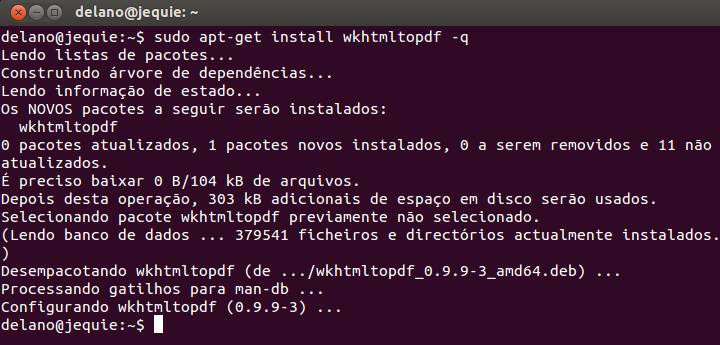
\includegraphics[width=12cm]{wkhtmltopdf}
\caption{Instalação do {\bf wkhtmltopdf}}
\label{figWkhtmltopdf}
\end{figure}

\newpage

\noindent{\bf  Configuração  de {\it  plugins}.}   Após  a  instalação dos  {\it
  plugins}  é   necessário  incluir   algumas  configurações  no   arquivo  {\bf
  conf/Config.groovy} (Código~\ref{codConfig}). Por questão de brevidade, apenas
serão apresentadas as mudanças realizadas nesse arquivo.  

\begin{itemize}

\vspace{0.3cm}

\item O primeiro bloco adiciona o  formato {\bf pdf} na lista de {\it MimeTypes}
  manipulados pela aplicação;

\vspace{0.3cm}

\item O segundo bloco configura a maneira em que os {\it scriptlets} (trechos de
  código)  são tratadas  nas  visões. Essa  alteração  é necessária  para o  bom
  funcionamento da geração de arquivos {\bf pdf};

\vspace{0.3cm}

\item Por fim,  o terceiro bloco indica onde  encontra-se instalada a ferramenta
  {\bf wkhtmltopdf}. 

\end{itemize}

\begin{lstlisting}[caption={\bf    Config.groovy},    frame=trBL,    float=htbp,
    label=codConfig]

grails.mime.types = [ // the first one is the default format
    all:           '*/*', // 'all' maps to '*' or the first available format in withFormat
    atom:          'application/atom+xml',
    css:           'text/css',
    csv:           'text/csv',
    pdf:           'application/x-pdf',
    form:          'application/x-www-form-urlencoded',
    html:          ['text/html','application/xhtml+xml'],
    js:            'text/javascript',
    json:          ['application/json', 'text/json'],
    multipartForm: 'multipart/form-data',
    rss:           'application/rss+xml',
    text:          'text/plain',
    hal:           ['application/hal+json','application/hal+xml'],
    xml:           ['text/xml', 'application/xml']
]

grails {
    views {
        gsp {
            encoding = 'UTF-8'
            htmlcodec = 'xml' // use xml escaping instead of HTML4 escaping
            codecs {
                expression = 'html' // escapes values inside ${}
                scriptlet = 'none' // escapes output from scriptlets in GSPs
                taglib = 'none' // escapes output from taglibs
                staticparts = 'none' // escapes output from static template parts
            }
        }
        // escapes all not-encoded output at final stage of outputting
        filteringCodecForContentType {
            //'text/html' = 'html'
        }
    }
}
 
grails.plugin.wkhtmltox.binary = "/usr/bin/wkhtmltopdf"
\end{lstlisting}

\section{Design responsivo}

\vspace{0.3cm}

Com  o objetivo  que  as  visões do  sistema  {\bf ControleBancario}  apresentem
leiautes  mais  responsivos,  essa  seção  descreve a  personalização  dos  {\it
  templates}  utilizados  pelo mecanismo  de  {\it  scaffolding}  na geração  de
visões.  É importante salientar que será utilizada, através do {\it plugin} {\bf
  pure-css}     instalado    anteriormente,     a     biblioteca    CSS     {\bf
  purecss}\footnote{\url{http://purecss.io}}  que  auxilia  no {\it  design}  de
leiautes responsivos.  
\index{Plugins!pure-css}

\subsection{Templates: create.gsp e edit.gsp}

\vspace{0.3cm}

Conforme discutido, o {\it template} {\bf create.gsp} é utilizado na geração das
visões {\bf  create} associadas  a cada um  dos controladores da  aplicação.  No
contexto desse  capítulo, esse  {\it template} será  alterado com o  objetivo de
utilizar  algumas   das  funcionalidades  providas  pela   biblioteca  CSS  {\bf
  purecss}. 

\begin{lstlisting}[numbers=left,        caption={\it        Template}       {\bf
      scaffolding/create.gsp}, frame = trBL,float=htbp, label=codTemCreate2]
<!DOCTYPE html>
<html>
 <head>
   <meta name="layout" content="main">       
   <g:set var="entityName" value="\${message(code:'${domainClass.propertyName}.label',default:'${className}')}" />
   <title><g:message code="default.create.label" args="[entityName]" /></title>
   <g:javascript src="jquery-1.8.3.min.js"/>
   <g:javascript src="jquery.maskedinput.min.js"/> 
   <g:javascript>
       var JQuery = jQuery.noConflict()
       JQuery(document).ready(function(){
         JQuery("#CPF").mask("999.999.999-99");
         JQuery("#CNPJ").mask("99.999.999/9999-99");
         JQuery("#CEP").mask("99999-999");
       });
   </g:javascript>
   <r:require module="pure-all" />
 </head>
 <body>
   <a href="#create-${domainClass.propertyName}" class="skip" tabindex="-1">
   <g:message code="default.link.skip.label" default="Skip to content&hellip;"/></a>
   <div class="pure-menu pure-menu-open pure-menu-horizontal">
     <ul>
      <li><a class="home" href="\${createLink(uri: '/')}"><g:message code="default.home.label"/></a></li>
      <li><g:link class="list" action="index"><g:message code="default.list.label" args="[entityName]" /> 
          </g:link></li>
      <li><g:link controller="logout">Logout</g:link></li>
     </ul>
   </div>
   <div id="create-${domainClass.propertyName}" class="content scaffold-create" role="main">
     <h1><g:message code="default.create.label" args="[entityName]" /></h1>
     <g:if test="\${flash.message}">
      <div class="message" role="status">\${flash.message}</div>
     </g:if>
     <g:hasErrors bean="\${${propertyName}}">
       <ul class="errors" role="alert">
        <g:eachError bean="\${${propertyName}}" var="error">
          <li <g:if test="\${error in org.springframework.validation.FieldError}">
               data-field-id="\${error.field}"</g:if>>
              <g:message error="\${error}"/></li>
        </g:eachError>
       </ul>
     </g:hasErrors>
     <g:form class="pure-form pure-form-aligned" url="[resource:${propertyName}, action:'save']" 
        <%= multiPart ? ' enctype="multipart/form-data"' : '' %>>
       <fieldset class="form">
         <g:render template="form"/>
       </fieldset>
       <fieldset class="buttons">
         <g:submitButton name="create" class="save" 
                        value="\${message(code: 'default.button.create.label', default: 'Create')}" />
       </fieldset>
     </g:form>
   </div>
 </body>
</html>
\end{lstlisting}

\newpage

\noindent  Código~\ref{codTemCreate2} mostra  as alterações  realizadas  no {\it
  template} {\bf create.gsp}: 

\begin{itemize}

\vspace{0.3cm}

\item A linha 7 adiciona a  folha de estilo (CSS), definida pela biblioteca {\bf
  purecss}, nas visões {\bf create} geradas pelo {\it scaffolding}; 

\vspace{0.3cm}

\item  As linhas  22 e  44 utilizam  os estilos  definidos pela  biblioteca {\bf
  purecss}  para adicionar  nas  visões, geradas  pelo  {\it scaffolding},  dois
  componentes HTML responsivos: um menu horizontal e um formulário; 

\vspace{0.3cm} 

\item Por  fim, a linha  27 adiciona uma  opção ao menu  horizontal, responsável
  pela operação de {\it logout} da aplicação.  

\end{itemize}

\vspace{0.3cm}

Análogo ao  {\bf create.gsp}, o  {\it template} {\bf edit.gsp}  também necessita
ser  alterado  com o  objetivo  de  utilizar  as funcionalidades  providas  pela
biblioteca  CSS {\bf  purecss}.  Código~\ref{codTemEdit2}  mostra  as alterações
realizadas  no {\it  template} {\bf  edit.gsp}.  Conforme  pode-se  observar, as
alterações são similares às realizadas no {\it template} {\bf create.gsp}.  

\begin{lstlisting}[numbers=left,        caption={\it        Template}       {\bf
      scaffolding/edit.gsp}, frame = trBL,float=htbp, label=codTemEdit2]
<%=packageName%>
<!DOCTYPE html>
<html>
  <head>
    <meta name="layout" content="main">
    <g:set var="entityName" value="\${message(code:'${domainClass.propertyName}.label',default:'${className}')}" />
    <title><g:message code="default.edit.label" args="[entityName]" /></title>
    <g:javascript src="jquery-1.8.3.min.js"/>
    <g:javascript src="jquery.maskedinput.min.js"/> 
    <g:javascript>
        var JQuery = jQuery.noConflict()
        JQuery(document).ready(function(){
          JQuery("#CPF").mask("999.999.999-99");
          JQuery("#CNPJ").mask("99.999.999/9999-99");
          JQuery("#CEP").mask("99999-999");
        });
    </g:javascript>
    <r:require module="pure-all" />
  </head>
  <body>
    <a href="#edit-${domainClass.propertyName}" class="skip" tabindex="-1">
    <g:message code="default.link.skip.label" default="Skip to content&hellip;"/></a>
    <div class="pure-menu pure-menu-open pure-menu-horizontal">
      <ul>
        <li><a class="home" href="\${createLink(uri: '/')}"><g:message code="default.home.label"/></a></li>
        <li><g:link class="list" action="index"><g:message code="default.list.label" args="[entityName]" />
            </g:link></li>
        <li><g:link class="create" action="create"><g:message code="default.new.label" args="[entityName]" />
            </g:link></li>
        <li><g:link controller="logout">Logout</g:link></li>
      </ul>
    </div>
    <div id="edit-${domainClass.propertyName}" class="content scaffold-edit" role="main">
      <h1><g:message code="default.edit.label" args="[entityName]" /></h1>
      <g:if test="\${flash.message}">
        <div class="message" role="status">\${flash.message}</div>
      </g:if>
      <g:hasErrors bean="\${${propertyName}}">
        <ul class="errors" role="alert">
          <g:eachError bean="\${${propertyName}}" var="error">
            <li <g:if test="\${error in org.springframework.validation.FieldError}">
                 data-field-id="\${error.field}"</g:if>><g:message error="\${error}"/></li>
          </g:eachError>
        </ul>
      </g:hasErrors>
      <g:form class="pure-form pure-form-aligned" url="[resource:${propertyName}, action:'update']" method="PUT" 
        <%= multiPart ? ' enctype="multipart/form-data"' : '' %>>
        <g:hiddenField name="version" value="\${${propertyName}?.version}" />
        <fieldset class="form">
          <g:render template="form"/>
        </fieldset>
        <fieldset class="buttons">
          <g:actionSubmit class="save" action="update" value="\${message(code: 'default.button.update.label', 
                                                                         default: 'Update')}" />
        </fieldset>
      </g:form>
    </div>
  </body>
</html>
\end{lstlisting}

\newpage

\subsection{Template: index.gsp}

\vspace{0.5cm}

Conforme discutido, o {\it template}  {\bf index.gsp} é utilizado na geração das
visões  {\bf index} associadas  a cada  um dos  controladores da  aplicação.  No
contexto desse  capítulo, esse  {\it template} será  alterado com o  objetivo de
utilizar  as  funcionalidades,  providas  pela  biblioteca  CSS  {\bf  purecss},
responsáveis  pela  obtenção  de  leiautes  mais  responsivos.  Por  questão  de
brevidade,  apenas   serão  apresentadas  as  mudanças   realizadas  nesse  {\it
  template}.  

\begin{lstlisting}[numbers=left,        caption={\it        Template}       {\bf
      scaffolding/index.gsp}, frame = trBL,float=htbp, label=codTemIndex2] 
<% import grails.persistence.Event %>
<%=packageName%>
<!DOCTYPE html>
<html>
   <head>
    <meta name="layout" content="main">
    <g:set var="entityName" value="\${message(code:'${domainClass.propertyName}.label',default:'${className}')}" />
    <title><g:message code="default.list.label" args="[entityName]" /></title>
    <r:require module="pure-all" />
   </head>
   <body>
     <a href="#list-${domainClass.propertyName}" class="skip" tabindex="-1">
     <g:message code="default.link.skip.label" default="Skip to content&hellip;"/></a>
      <div class="pure-menu pure-menu-open pure-menu-horizontal">
       <ul>
        <li><a class="home" href="\${createLink(uri: '/')}"><g:message code="default.home.label"/></a></li>
        <li>
          <sec:access controller="${domainClass.propertyName}" action='create'>
            <g:link class="create" action="create"><g:message code="default.new.label" args="[entityName]" />
            </g:link>
          </sec:access>
         </li>
         <li><g:link controller="logout">Logout</g:link></li> 
       </ul>
       </div>
       <div id="list-${domainClass.propertyName}" class="content scaffold-list" role="main">
         <h1><g:message code="default.list.label" args="[entityName]" /></h1>
          <g:if test="\${flash.message}">
            <div class="message" role="status">\${flash.message}</div>
          </g:if>
          <table class="pure-table pure-table-bordered">
          
          <!-- Defini^çã^o da tabela -- Removido por quest^õ^es de brevidade --> 

          </table>
          <div class="pagination">
           <g:paginate total="\${${propertyName}Count ?: 0}" />
          </div>
       </div>
   </body>
</html>
\end{lstlisting}

\noindent  Código~\ref{codTemIndex2}  mostra as  alterações  realizadas no  {\it
  template} {\bf index.gsp}: 

\begin{itemize}

\vspace{0.5cm}

\item A linha 9 adiciona a  folha de estilo (CSS), definida pela biblioteca {\bf
  purecss}, nas visões {\bf index} geradas pelo {\it scaffolding}; 

\vspace{0.5cm}

\item  As linhas  14 e  31 utilizam  os estilos  definidos pela  biblioteca {\bf
  purecss}  para adicionar  nas  visões, geradas  pelo  {\it scaffolding},  dois
  componentes HTML responsivos: um menu horizontal e uma tabela; e

\vspace{0.5cm} 

\item Por  fim, a linha  23 adiciona uma  opção ao menu  horizontal, responsável
  pela operação de {\it logout} da aplicação.  

\end{itemize}

\newpage

\subsection{Template: show.gsp}

\vspace{0.5cm}

Conforme discutido, o  {\it template} {\bf show.gsp} é  utilizado na geração das
visões  {\bf show}  associadas a  cada um  dos controladores  da  aplicação.  No
contexto desse  capítulo, esse  {\it template} será  alterado com o  objetivo de
utilizar  as  funcionalidades,  providas  pela  biblioteca  CSS  {\bf  purecss},
responsáveis  pela  obtenção  de  leiautes  mais responsivos.   Por  questão  de
brevidade, apenas serão apresentadas as mudanças realizadas nesse {\it template}.

\begin{lstlisting}[numbers=left,        caption={\it        Template}       {\bf
      scaffolding/show.gsp}, frame = trBL,float=htbp, label=codTemShow2] 
<% import grails.persistence.Event %>
<%=packageName%>
<!DOCTYPE html>
<html>
  <head>
    <meta name="layout" content="main">
    <g:set var="entityName" value="\${message(code:'${domainClass.propertyName}.label',default:'${className}')}"/>
    <title><g:message code="default.show.label" args="[entityName]" /></title>
    <r:require module="pure-all" />
  </head>
  <body>
    <a href="#show-${domainClass.propertyName}" class="skip" tabindex="-1"><g:message 
                     code="default.link.skip.label" default="Skip to content&hellip;"/></a>
    <div class="pure-menu pure-menu-open pure-menu-horizontal">
     <ul>
      <li><a class="home" href="\${createLink(uri: '/')}"><g:message code="default.home.label"/></a></li>
      <li><g:link class="list" action="index"><g:message code="default.list.label" args="[entityName]"/></g:link>
      </li><li>
       <sec:access controller="${domainClass.propertyName}" action='create'>
        <g:link class="create" action="create"><g:message code="default.new.label" args="[entityName]" /></g:link>
       </sec:access>
      </li>
      <li><g:link controller="logout">Logout</g:link></li>
     </ul>
    </div>

    <!-- Defini^çã^o das demais tags -- Removido por quest^õ^es de brevidade -->    

  </body>
</html>
\end{lstlisting}

\noindent  Código~\ref{codTemShow2}  mostra as  alterações realizadas  no {\it
  template} {\bf show.gsp}: 

\begin{itemize}

\vspace{0.5cm}

\item A linha 9 adiciona a  folha de estilo (CSS), definida pela biblioteca {\bf
  purecss}, nas visões {\bf index} geradas pelo {\it scaffolding}; 

\vspace{0.5cm}

\item A linha 14 utiliza os estilos definidos pela biblioteca {\bf purecss} para
  adicionar  nas visões,  geradas  pelo {\it  scaffolding},  um componente  HTML
  responsivo: um menu horizontal; 

\vspace{0.5cm} 

\item Por  fim, a linha  23 adiciona uma  opção ao menu  horizontal, responsável
  pela operação de {\it logout} da aplicação.  

\end{itemize}

\subsection{Biblioteca de marcas: LoginTagLib}

\vspace{0.5cm}

Conforme discutido  anteriormente, os {\it  templates} adicionaram uma  opção ao
menu horizontal, responsável  pela operação de {\it logout}  da aplicação. Dessa
forma,   Código~\ref{codTagLib3}   apresenta  a   biblioteca   de  marcas   {\bf
  LoginTagLib}  que foi  reimplementada para  refletir as  alterações discutidas
nesse capítulo:  remoção do {\it link}  para o controlador {\bf  Logout} -- essa
opção agora encontra-se  presente no menu horizontal de  todas as visões geradas
pelo {\it scaffolding}.  

\begin{lstlisting}[caption=Biblioteca  de marca  {\bf  LoginTagLib}, frame=trBL,
    float=htbp, label=codTagLib3, numbers=left] 
class LoginTagLib {
    def springSecurityService
    def loginControl = {
        if (springSecurityService.isLoggedIn()) {
            def usuario = springSecurityService.getCurrentUser() 
            def authority = usuario.getAuthorities()[0].getAuthority()
            def papel
            
            def span = "<span style=\"text-align:center;padding-left:25px;padding-right:25px\">"
            
            StringBuilder sb = new StringBuilder();
            
            if (session.contaCliente) {
                sb.append("Conta: ")
                sb.append(session.contaCliente.conta)
                sb.append(" [")
                sb.append(session.contaCliente.conta.agencia)
                sb.append("]")
                sb.append(span)
            } else if (session.agencia) { 
                sb.append("Ag^ê^ncia: ")
                sb.append(session.agencia)
            }
            
            out << span
            out << session.papel
            out << "</span>"
            out << span
            out << sb
            out << "</span>"
        }
    }
}
\end{lstlisting}

\subsection{Visões: geração automática pelo mecanismo de {\it Scaffolding}}

\vspace{0.5cm}

Após  realizar as  alterações  discutidas nas  seções  anteriores, é  necessário
executar  o  comando  {\bf  generate-views}  para que  as  alterações  nos  {\it
  templates}, discutidos  na seções anteriores,  sejam refletidos nas  visões da
aplicação  {\bf ControleBancario}.  No  IDE GGTS:  Selecione {\bf  Grails Tools}
$\Longrightarrow$ {\bf Grails Command Wizard}.  Digite {\bf generate-views} como
o  nome do  comando a  ser executado  e  clique em  {\bf Next}.   Digite o  nome
da  classe de  domínio  como o  parâmetro do  comando  e clique  em {\bf  Next}.
Tabela~\ref{tblGenerateAll} lista  o nome das classes de  domínio que necessitam
que as visões sejam geradas novamente.
\index{Comandos!grails generate-views} 

\vspace{0.5cm}

\noindent{\bf  Observação:} Os  {\it templates}  {\bf \_form.gsp},  associados a
cada uma  das classes de domínio,  não precisam ser gerados  novamente. Ou seja,
digite a opção {\bf n} para o  {\it template} {\bf \_form.gsp} e {\bf y} para as
demais  visões.  Figura~\ref{figGenerateViews}  apresenta a  geração  das visões
associadas a classe de domínio {\bf br.ufscar.dc.dsw.Agencia}.  

\vspace{0.3cm}

\begin{figure}[htbp]
\centering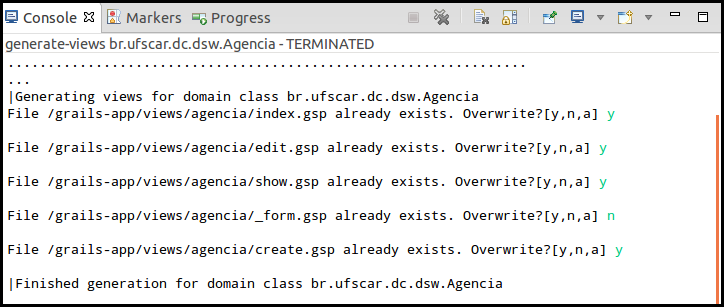
\includegraphics[width=12cm]{generateViews}
\caption{Comando {\bf grails generate-views}}
\label{figGenerateViews}
\end{figure}

\newpage

\section{Personalização dos atributos (Cliente Físico/Jurídico e Gerente)}

\vspace{0.3cm}

Conforme  discutido as  classes de  domínio {\bf  Cliente} e  {\bf  Gerente} são
subclasses da classe {\bf Usuario}  que provê as funcionalidades relacionadas ao
controle  de  acesso.   Dessa  forma,  eles  herdam  alguns  atributos  que  são
específicos às funcionalidades de controle de acesso ({\bf accountExpired}, {\bf
  accountLocked},  etc). Visando  ``despoluir'' (removendo  esses  atributos) as
visões, relacionadas  a essas classes de domínio,  serão personalizadas conforme
será discutido nessa seção. 

Em  adição, essa  seção discute  a utilização  da {\it  tag}  {\bf dateChooser},
definida  pelo  {\it plugin}  {\bf  richui},  na  personalização da  entrada  de
atributos que representam datas (ver Figura~\ref{calendarFig}).

\begin{figure}[htbp]
\centering
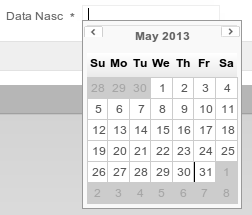
\includegraphics[width=5cm]{calendar}
\caption{Calendário dinâmico: {\bf <richui: dataChooser />}}
\label{calendarFig}
\end{figure}

\subsection{Cliente Físico, Cliente Jurídico e Gerente}

\vspace{0.3cm}

Código~\ref{codClienteCreate2}  apresenta a  alteração (linha  16)  realizada na
visão {\bf clienteFisico/create.gsp} com o  objetivo de permitir a utilização da
{\it tag} {\bf  dateChooser} na entrada de atributos  que representam datas. Por
questão de  brevidade, apenas será  apresentada a única mudança  realizada nesse
arquivo.  

 \begin{lstlisting}[numbers=left,  caption=Visão {\bf clienteFisico/create.gsp},
     frame=trBL, float=htbp, label=codClienteCreate2] 
<html>
 <head>
  <meta name="layout" content="main">
  <g:set var="entityName" value="${message(code: 'clienteFisico.label', default: 'ClienteFisico')}" />
  <title><g:message code="default.create.label" args="[entityName]" /></title>
  <g:javascript src="jquery-1.8.3.min.js"/>
  <g:javascript src="jquery.maskedinput.min.js"/> 
  <g:javascript>
      var JQuery = jQuery.noConflict()
      JQuery(document).ready(function(){
          JQuery("#CPF").mask("999.999.999-99");
          JQuery("#CNPJ").mask("99.999.999/9999-99");
          JQuery("#CEP").mask("99999-999");
      });
  </g:javascript>
  <resource:dateChooser />
  <r:require module="pure-all" />
 </head>
 <body>

 <!-- Defini^çã^o das demais tags -- Removido por quest^õ^es de brevidade --> 

 </body>
</html>
\end{lstlisting}

\vspace{0.3cm}

\begin{remark}
Análogo    à   visão    {\bf   clienteFisico/create.gsp},    as    visões   {\bf
  clienteFisico/edit.gsp},     {\bf    clienteJuridico/create.gsp}     e    {\bf
  clienteJuridico/edit.gsp}  também  necessitam ser  alteradas  para permitir  a
utilização  da  {\it  tag}  {\bf   dateChooser}  na  entrada  de  atributos  que
representam datas.  Fica como exercício para o leitor realizar tais alterações.  
\end{remark}

\newpage

\noindent  Código~\ref{codClienteFisicoForm2} apresenta  o  {\it template}  {\bf
  clienteFisico/\_form.gsp} que  foi reimplementado para  refletir as alterações
discutidas  nesse capítulo: remoção  dos atributos  {\bf accountExpired}  e {\bf
  accountLocked}.   Além disso,  esse {\it  template} utiliza  a {\it  tag} {\bf
  dateChooser}  (linha 31)  definido pelo  {\it plugin}  {\bf  richui} instalado
anteriormente. 

\vspace{0.3cm}

\begin{lstlisting}[numbers=left,        caption={\it        Template}       {\bf
      clienteFisico/\_form.gsp},             frame=trBL,             float=htbp,
    label=codClienteFisicoForm2] 
<%@ page import="br.ufscar.dc.dsw.ClienteFisico" %>
<div class="fieldcontain ${hasErrors(bean: clienteFisicoInstance, field: 'username', 'error')} required">
	<label for="username">
		<g:message code="clienteFisico.username.label" default="Username" />
	</label>
	<g:textField name="username" required="" value="${clienteFisicoInstance?.username}"/>
</div>
<div class="fieldcontain ${hasErrors(bean: clienteFisicoInstance, field: 'password', 'error')} required">
	<label for="password">
		<g:message code="clienteFisico.password.label" default="Password" />
	</label>
	<g:field type="password" name="password" required="" value="${clienteFisicoInstance?.password}"/>
</div>
<div class="fieldcontain ${hasErrors(bean: clienteFisicoInstance, field: 'nome', 'error')} required">
	<label for="nome">
		<g:message code="clienteFisico.nome.label" default="Nome" />
	</label>
	<g:textField name="nome" maxlength="30" required="" value="${clienteFisicoInstance?.nome}"/>
</div>
<div class="fieldcontain ${hasErrors(bean: clienteFisicoInstance, field: 'endereco', 'error')} required">
	<label for="endereco">
		<g:message code="clienteFisico.endereco.label" default="Endereco" />
	</label>
	<g:select id="endereco" name="endereco.id" from="${br.ufscar.dc.dsw.Endereco.list()}" optionKey="id" 
            required="" value="${clienteFisicoInstance?.endereco?.id}" class="many-to-one"/>
</div>
<div class="fieldcontain ${hasErrors(bean: clienteFisicoInstance, field: 'dtMoradia', 'error')} required">
	<label for="dtMoradia">
		<g:message code="clienteFisico.dtMoradia.label" default="Dt Moradia" />
	</label>
  <richui:dateChooser name="dtMoradia" format="dd/MM/yyyy" value="${clienteFisicoInstance?.dtMoradia}"/>
</div>
<div class="fieldcontain ${hasErrors(bean: clienteFisicoInstance, field: 'status', 'error')} required">
	<label for="status">
		<g:message code="clienteFisico.status.label" default="Status" />
	</label>
	<g:select name="status" from="${clienteFisicoInstance.constraints.status.inList}" required="" 
            value="${clienteFisicoInstance?.status}" valueMessagePrefix="clienteFisico.status"/>
</div>
<div class="fieldcontain ${hasErrors(bean: clienteFisicoInstance, field: 'rg', 'error')} required">
	<label for="rg">
		<g:message code="clienteFisico.rg.label" default="Rg" />
	</label>
	<g:textField name="rg" maxlength="12" required="" value="${clienteFisicoInstance?.rg}"/>
</div>

<div class="fieldcontain ${hasErrors(bean: clienteFisicoInstance, field: 'CPF', 'error')} required">
	<label for="CPF">
		<g:message code="clienteFisico.CPF.label" default="CPF" />
	</label>
	<g:textField name="CPF" maxlength="14" required="" value="${clienteFisicoInstance?.CPF}"/>
</div>
<div class="fieldcontain ${hasErrors(bean: clienteFisicoInstance, field: 'contasCliente', 'error')} ">
	<label for="contasCliente">
		<g:message code="clienteFisico.contasCliente.label" default="Contas Cliente" />		
	</label>
	
<ul class="one-to-many">
<g:each in="${clienteFisicoInstance?.contasCliente?}" var="c">
    <li><g:link controller="contaCliente" action="show" id="${c.id}">${c?.encodeAsHTML()}</g:link></li>
</g:each>
<li class="add">
  <g:link controller="contaCliente" action="create" params="['clienteFisico.id': clienteFisicoInstance?.id]">
     ${message(code: 'default.add.label', args: [message(code: 'contaCliente.label', default: 'ContaCliente')])}
  </g:link>
</li>
</ul>
</div>
\end{lstlisting}

\vspace{0.3cm}

\begin{remark}
Análogo  ao {\it  template} {\bf  clienteFisico/\_form.gsp}, os  {\it templates}
{\bf  clienteJuridico/\_form.gsp} e  {\bf gerente/\_form.gsp}  também necessitam
ser alteradas.  Fica como exercício para o leitor realizar tais alterações.  
\end{remark}

\newpage

\noindent    Código~\ref{codClienteFisicoIndex2}   apresenta   a    visão   {\bf
  clienteFisico/index.gsp}  que foi reimplementada  para refletir  as alterações
discutidas nesse  capítulo: a personalização dos atributos  a serem apresentados
nas visões. 

\vspace{0.5cm}

\begin{lstlisting}[numbers=left,  caption=Visão  {\bf  clienteFisico/index.gsp},
    frame=trBL, float=htbp, label=codClienteFisicoIndex2] 

<%@ page import="br.ufscar.dc.dsw.ClienteFisico" %>
<!DOCTYPE html>
<html>
  <head>
    <meta name="layout" content="main">
    <g:set var="entityName" value="${message(code: 'clienteFisico.label', default: 'ClienteFisico')}" />
    <title><g:message code="default.list.label" args="[entityName]" /></title>
    <r:require module="pure-all" />
  </head>
  <body>
    <a href="#list-clienteFisico" class="skip" tabindex="-1">
    <g:message code="default.link.skip.label" default="Skip to content&hellip;"/></a>
    <div class="pure-menu pure-menu-open pure-menu-horizontal">
     <ul>
      <li><a class="home" href="${createLink(uri: '/')}"><g:message code="default.home.label"/></a></li>
      <li><sec:access controller="clienteFisico" action='create'>
            <g:link class="create" action="create"><g:message code="default.new.label" args="[entityName]" />
            </g:link>
           </sec:access>
      </li>                            
      <li><g:link controller="logout">Logout</g:link></li>
     </ul>
    </div>
    <div id="list-clienteFisico" class="content scaffold-list" role="main">
      <h1><g:message code="default.list.label" args="[entityName]" /></h1>
      <g:if test="${flash.message}">
        <div class="message" role="status">${flash.message}</div>
      </g:if>
      <table class="pure-table pure-table-bordered">
        <thead>
          <tr>
            <g:sortableColumn property="nome" title="${message(code:'clienteFisico.nome.label',default:'Nome')}" />
            <th><g:message code="clienteFisico.endereco.label" default="Endereco" /></th>
            <g:sortableColumn property="dtMoradia" title="${message(code: 'clienteFisico.dtMoradia.label', 
                                                                    default: 'Dt Moradia')}" />
            <g:sortableColumn property="status" title="${message(code: 'clienteFisico.status.label', 
                                                                 default: 'Status')}" />
          </tr>
        </thead>
        <tbody>
          <g:each in="${clienteFisicoInstanceList}" status="i" var="clienteFisicoInstance">
            <tr class="${(i % 2) == 0 ? 'even' : 'odd'}">
              <td><g:link action="show" id="${clienteFisicoInstance.id}">
                  ${fieldValue(bean: clienteFisicoInstance, field: "nome")}</g:link></td>
              <td>${fieldValue(bean: clienteFisicoInstance, field: "endereco")}</td>
              <td><g:formatDate date="${clienteFisicoInstance.dtMoradia}" /></td>
              <td>${fieldValue(bean: clienteFisicoInstance, field: "status")}</td>
            </tr>
          </g:each>
        </tbody>
      </table>
      <div class="pagination">
        <g:paginate total="${clienteFisicoInstanceCount ?: 0}" />
      </div>
    </div>
  </body>
</html>
\end{lstlisting}

\vspace{0.5cm}

\begin{remark}
Análogo    à    visão   {\bf    clienteFisico/index.gsp},    as   visões    {\bf
  clienteFisico/show.gsp},       {\bf      clienteJuridico/index.gsp},      {\bf
  clienteJuridico/show.gsp},  {\bf gerente/index.gsp}  e  {\bf gerente/show.gsp}
também necessitam  ser alterados com o  objetivo de personalizar  os atributos a
serem apresentados. Fica como exercício para o leitor realizar tais alterações.  
\end{remark}

\newpage

\subsection{Cliente}

\vspace{0.5cm}

Conforme  discutido   anteriormente,  a  classe  de  domínio   {\bf  Cliente}  é
abstrata.  Portanto, as  visões  associadas a  essa  classe de  domínio não  são
geradas  automaticamente pelo  mecanismo  de {\it  scaffolding}.   A visão  {\bf
  cliente/index.gsp} apresenta uma lista de clientes.  Código~\ref{codCliIndex2}
apresenta a reimplementação dessa visão com o objetivo da obtenção de um leiaute
mais  responsivo: menu  horizontal (linha  14), formulário  (linha 25)  e tabela
(linha 37).  

Adicionamente,    essa    visão     disponibiliza    a    funcionalidade    {\it
  autocomplete}. Além  de ser visualmente  mais agradável, este recurso  faz com
que apenas apareçam as opções de acordo  com o que é digitado em um campo texto.
Para a aplicação {\bf ControleBancario}, a funcionalidade {\it autocomplete} foi
utilizada objetivando  auxiliar a busca  de clientes (físicos ou  jurídicos).  A
funcionalidade   {\it  autocomplete}   é  implementada   pela  {\it   tag}  {\bf
  autocomplete}  (linhas   30-32)  do   {\it  plugin}  {\bf   richui}  instalado
anteriormente.  

\begin{lstlisting}[numbers=left,  caption=Visão  {\bf cliente/index.gsp},  frame
    =trBL,float=htbp, label=codCliIndex2]
<%@ page import="br.ufscar.dc.dsw.Cliente" %>
<!DOCTYPE html>
<html>
 <head>
  <meta name="layout" content="main">
  <g:set var="entityName" value="${message(code: 'cliente.label', default: 'Cliente')}" />
  <title><g:message code="default.list.label" args="[entityName]" /></title>
  <resource:autoComplete skin="default" />
  <r:require module="pure-all" />
 </head>
 <body>
  <a href="#list-cliente" class="skip" tabindex="-1">
  <g:message code="default.link.skip.label" default="Skip to content&hellip;"/></a>
  <div class="pure-menu pure-menu-open pure-menu-horizontal">
   <ul>
    <li><a class="home" href="${createLink(uri: '/')}"><g:message code="default.home.label"/></a></li>
    <li><g:link controller="logout">Logout</g:link></li>
   </ul>
  </div>
  <div id="list-cliente" class="content scaffold-list" role="main">
   <h1><g:message code="default.list.label" args="[entityName]" /></h1>
    <g:if test="${flash.message}">
     <div class="message" role="status">${flash.message}</div>
    </g:if>
    <form class="pure-form">
     <table>
      <thead>
       <th> <g:message code="search.label"/> </th>
       <th>
        <richui:autoComplete name="search"
          onItemSelect="document.location.href = '${createLinkTo(dir: 'cliente/show')}/' + id;" 
          class="pure-input-rounded" action="${createLinkTo('dir': 'cliente/searchAJAX')}"/>
       </th>
      </thead> 
     </table>
    </form>
    <table class="pure-table pure-table-bordered">
     <thead>
      <tr><g:sortableColumn property="nome" title="${message(code: 'cliente.nome.label', default: 'Nome')}" />
      <th><g:message code="cliente.endereco.label" default="Endereco" /></th>
      <g:sortableColumn property="dtMoradia" title="${message(code: 'cliente.dtMoradia.label', 
                                                              default: 'Dt Moradia')}" />
      <g:sortableColumn property="status" title="${message(code: 'cliente.status.label', 
                                                           default: 'Status')}" /></tr>
     </thead>
     <tbody>
      <g:each in="${list}" status="i" var="clienteInstance">
       <tr class="${(i % 2) == 0 ? 'even' : 'odd'}">
       <td><g:link action="show" id="${clienteInstance.id}">
           ${fieldValue(bean: clienteInstance, field: "nome")}</g:link></td>
       <td>${fieldValue(bean: clienteInstance, field: "endereco")}</td>
       <td><g:formatDate date="${clienteInstance.dtMoradia}" /></td>
       <td>${fieldValue(bean: clienteInstance, field: "status")}</td></tr>
      </g:each>
     </tbody>
    </table>
    <div class="pagination">
     <g:paginate total="${clienteInstanceCount ?: 0}" />
    </div>
  </div>
 </body>
</html>
\end{lstlisting}

\newpage

\noindent  Conforme pode-se  observar, a  {\it tag}  {\bf <richui:autoComplete>}
(linhas 30-32) invoca assincronamente (sempre  que ocorre uma edição no campo de
texto   {\bf   search})   a   ação   {\bf  searchAJAX}   do   controlador   {\bf
  ClienteController}  que realiza  uma  busca nos  clientes  baseando-se no  que
encontra-se  digitado  no  campo  texto   e  retorna  as  opções  possíveis.   A
implementação da ação {\bf  searchAJAX} do controlador {\bf ClienteController} é
apresentada no Código~\ref{codClienteController2}.  

\begin{lstlisting}[caption=Controlador          {\bf         ClienteController},
    frame=trBL,float=htbp, label=codClienteController2]
class ClienteController {

    // Demais a^çõ^es/atributos/m^é^todos do controlador ClienteController
    
    def searchAJAX () {
        
        // busca clientes
        def clientes = Cliente.findAllByNomeLike("%${params.query}%")
        //  cria resposta XML
        render(contentType: "text/xml") { // retorna os clientes encontrados
            results() { 
                clientes.each { 
                    cliente ->result() {
                        name(cliente.nome)
                        id (cliente.id)
                    }
                }
            }
        }
    }
}
\end{lstlisting}

\noindent  Figura~\ref{autocompleteFig} (A)  ilustra a  situação onde  o usuário
digitou 'e'. Nesse caso, os dois clientes estão presentes nas opções disponíveis
desde que  a sentença 'e'  encontra-se presente nos  nomes dos dois  clientes --
P\underline{e}dro Soares e Viação Com\underline{e}ta S/A. 

\vspace{0.2cm}

\begin{figure}[htbp]
\center
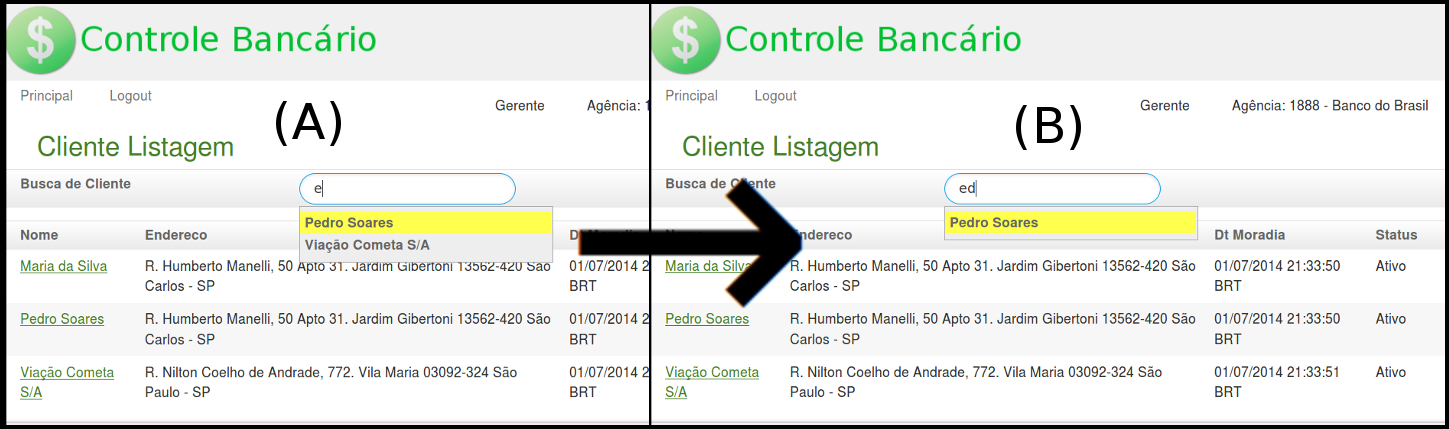
\includegraphics[width=15cm]{autocomplete}
\caption{Funcionalidade {\it autocomplete} -- Busca de clientes}
\label{autocompleteFig}
\end{figure}

\vspace{0.2cm}

\noindent  Figura~\ref{autocompleteFig} (B)  ilustra a  situação onde  o usuário
digitou 'ed'. Nesse caso, apenas um cliente está presente nas opções disponíveis
desde que a  sentença 'ed' encontra-se presente no nome de  apenas um cliente --
P\underline{ed}ro  Soares. Ao selecionar  essa opção,  a aplicação  apresenta as
informações  desse  cliente  (invoca  a  ação {\bf  show}  do  controlador  {\bf
  Cliente}).  

\newpage

\section{Personalização das visões: Contas (corrente \& poupança)}
\index{Plugins!richui}

\vspace{0.5cm}

Essa seção  discute a utilização da  {\it tag} {\bf  dateChooser}, definida pelo
{\it  plugin} {\bf  richui},  na  personalização da  entrada  de atributos  (que
representam datas) das classes de domínio que representam contas bancárias. 

Código~\ref{codCorrenteCreate2}  apresenta a  alteração (linha  16)  realizada na
visão {\bf contaCorrente/create.gsp} com o  objetivo de permitir a utilização da
{\it tag} {\bf  dateChooser} na entrada de atributos  que representam datas. Por
questão de  brevidade, apenas será  apresentada a única mudança  realizada nesse
arquivo.  

\vspace{0.3cm}

 \begin{lstlisting}[numbers=left,  caption=Visão {\bf contaCorrente/create.gsp},
     frame=trBL, float=htbp, label=codCorrenteCreate2] 
<html>
 <head>
  <meta name="layout" content="main">
  <g:set var="entityName" value="${message(code: 'contaCorrente.label', default: 'ContaCorrente')}" />
  <title><g:message code="default.create.label" args="[entityName]" /></title>
  <g:javascript src="jquery-1.8.3.min.js"/>
  <g:javascript src="jquery.maskedinput.min.js"/> 
  <g:javascript>
      var JQuery = jQuery.noConflict()
      JQuery(document).ready(function(){
          JQuery("#CPF").mask("999.999.999-99");
          JQuery("#CNPJ").mask("99.999.999/9999-99");
          JQuery("#CEP").mask("99999-999");
      });
  </g:javascript>
  <resource:dateChooser />
  <r:require module="pure-all" />
 </head>
 <body>

 <!-- Defini^çã^o das demais tags -- Removido por quest^õ^es de brevidade --> 

 </body>
</html>
\end{lstlisting}

\begin{remark}
Análogo    à   visão    {\bf   contaCorrente/create.gsp},    as    visões   {\bf
  contaCorrente/edit.gsp},     {\bf     contaPoupanca/create.gsp}     e     {\bf
  contaPoupanca/edit.gsp}  também  necessitam  ser  alteradas  para  permitir  a
utilização  da  {\it  tag}  {\bf   dateChooser}  na  entrada  de  atributos  que
representam datas.  Fica como exercício para o leitor realizar tais alterações.  
\end{remark}

\vspace{0.3cm}

\noindent   Código~\ref{codCorrenteForm2}   mostra   o   {\it   template}   {\bf
  contaCorrente/\_form.gsp} que  foi reimplementado para  refletir as alterações
discutidas nesse  capítulo: utilização da {\it tag}  {\bf dateChooser}, definida
pelo  {\it plugin}  {\bf richui},  na entrada  de valores  para o  atributo {\bf
  abertura} da classe de domínio {\bf ContaCorrente}.  

\vspace{0.3cm}

\begin{lstlisting}[caption={\it    Template}   {\bf   contaCorrente/\_form.gsp},
    frame=trBL, float=htbp, label=codCorrenteForm2] 
<%@ page import="br.ufscar.dc.dsw.ContaCorrente" %>

 <!-- Defini^çã^o das demais tags -- Removido por quest^õ^es de brevidade -->

<div class="fieldcontain ${hasErrors(bean: contaCorrenteInstance, field: 'abertura', 'error')} required">
  <label for="abertura">
    <g:message code="contaCorrente.abertura.label" default="Abertura" />
    <span class="required-indicator">*</span>
  </label>
  <richui:dateChooser name="abertura" format="dd/MM/yyyy" value="${contaCorrenteInstance?.abertura}"/>
</div>

 <!-- Defini^çã^o das demais tags -- Removido por quest^õ^es de brevidade -->

\end{lstlisting}

\begin{remark}
Análogo ao {\it template}  {\bf contaCorrente/\_form.gsp}, o {\it template} {\bf
  contaPoupanca/\_form.gsp} também necessita  ser alterado.  Fica como exercício
para o leitor realizar tais alterações.  
\end{remark}

\newpage

\subsection{Visão: conta/index.gsp}

\vspace{0.5cm}

Conforme discutido  anteriormente, a classe  de domínio {\bf Conta}  é abstrata.
Portanto,  as  visões  associadas a  essa  classe  de  domínio não  são  geradas
automaticamente   pelo   mecanismo   de   {\it  scaffolding}.   A   visão   {\bf
  conta/index.gsp} apresenta  uma lista de  contas bancárias (não  importando se
estas são contas correntes ou poupanças).  Código~\ref{codContaIndex2} apresenta
a reimplementação  dessa visão  com o  objetivo da obtenção  de um  leiaute mais
responsivo: menu horizontal  (linha 13) e tabela (linha  24).  Em complemento, a
linha 16  adiciona uma  opção ao menu  horizontal, responsável pela  operação de
{\it logout} da aplicação.  

\begin{lstlisting}[numbers=left,  caption=Visão  {\bf conta/index.gsp},  frame
    =trBL,float=htbp, label=codContaIndex2]
<%@ page import="br.ufscar.dc.dsw.Conta" %>
<!DOCTYPE html>
<html>
 <head>
   <meta name="layout" content="main">
   <g:set var="entityName" value="${message(code: 'conta.label', default: 'Conta')}" />
   <title><g:message code="default.list.label" args="[entityName]" /></title>
   <r:require module="pure-all" />
 </head>
 <body>
   <a href="#list-conta" class="skip" tabindex="-1">
   <g:message code="default.link.skip.label" default="Skip to content&hellip;"/></a>
   <div class="pure-menu pure-menu-open pure-menu-horizontal">
     <ul>
       <li><a class="home" href="${createLink(uri: '/')}"><g:message code="default.home.label"/></a></li>
       <li><g:link controller="logout">Logout</g:link></li>
     </ul>
   </div>
   <div id="list-conta" class="content scaffold-list" role="main">
     <h1><g:message code="default.list.label" args="[entityName]" /></h1>
     <g:if test="${flash.message}">
       <div class="message" role="status">${flash.message}</div>
     </g:if>
     <table class="pure-table pure-table-bordered">
       <thead>
         <tr>
           <th><g:message code="conta.agencia.label" default="Agencia" /></th>
           <g:sortableColumn property="numero" title="${message(code: 'conta.numero.label', default: 'Numero')}" />
           <g:sortableColumn property="saldo" title="${message(code: 'conta.saldo.label', default: 'Saldo')}" />
           <g:sortableColumn property="abertura" title="${message(code: 'conta.abertura.label', 
                                                                  default: 'Abertura')}" />
         </tr>
       </thead>
       <tbody>
         <g:each in="${list}" status="i" var="contaInstance">
           <tr class="${(i % 2) == 0 ? 'even' : 'odd'}">
             <td><g:link action="show" id="${contaInstance.id}">
                   ${fieldValue(bean: contaInstance, field: "agencia")}</g:link></td>
             <td>${fieldValue(bean: contaInstance, field: "numero")}</td>
             <td>${fieldValue(bean: contaInstance, field: "saldo")}</td>
             <td><g:formatDate date="${contaInstance.abertura}" /></td>
           </tr>
         </g:each>
       </tbody>
     </table>
     <div class="pagination">
       <g:paginate total="${contaInstanceCount ?: 0}" />
     </div>
   </div>
 </body>
</html>
\end{lstlisting}

\section{Visões: main/index.gsp \& selecionaConta/index.gsp}

\vspace{0.5cm}

Relembrando   a   discussão  do   Capítulo~\ref{autenticacao},   a  visão   {\bf
  main/index.gsp}    consiste   na   visão    principal   da    aplicação   {\bf
  ControleBancario}.   Código~\ref{codMainIndex2}  apresenta  a  reimplementação
dessa  visão com  o objetivo  da obtenção  de um  leiaute mais  responsivo: menu
horizontal (linha  9) e menu  vertical (linha 14).   Em complemento, a  linha 11
adiciona uma opção ao menu horizontal, responsável pela operação de {\it logout}
da aplicação.  

\begin{lstlisting}[numbers=left, caption=Visão {\bf main/index.gsp}, frame=trBL,
    float=htbp, label=codMainIndex2]
<!DOCTYPE html>
<html>
 <head>
   <meta name="layout" content="main">
   <g:javascript library="jquery" />
   <r:require module="pure-all" />
 </head>
 <body>
  <div class="pure-menu pure-menu-open pure-menu-horizontal">
   <ul><li><a class="home" href="${createLink(uri: '/')}"><g:message code="default.home.label"/></a></li>
       <li><g:link controller="logout">Logout</g:link></li></ul>
  </div>
  <h2><g:message code="main.options"/></h2>
  <div class="pure-menu pure-menu-open">
   <ul>
    <g:each var="c" in="${grailsApplication.controllerClasses.sort { it.fullName } }">
     <g:set var="name" value="${c.logicalPropertyName}" />
     <g:if test="${name != 'logout' && name != 'login' && name != 'main'}">
      <sec:access url='${createLink(controller: c.logicalPropertyName, base: "/")}'>
       <li><g:link controller="${c.logicalPropertyName}">${c.naturalName.replace("Controller","")}</g:link></li>
      </sec:access>
     </g:if>
    </g:each>
   </ul>
  </div>
 </body>
</html>
\end{lstlisting}

\vspace{0.5cm}

\noindent Relembrando  a discussão  do Capítulo~\ref{autorizacao}, se  o cliente
          {\it logado}  possui mais de uma  conta (corrente ou  poupança), a ele
          será  solicitado  escolher  que   conta  ele  deseja  acessar.   Nesse
          contexto, a visão {\bf selecionaConta/index.gsp} apresenta um campo de
          seleção  que  contém as  contas  associadas  ao  cliente {\it  logado}
          (variável                 de                sessão                {\bf
            cliente}).    Código~\ref{codSelecionaContaIndex2}    apresenta    a
          reimplementação dessa visão  com o objetivo da obtenção  de um leiaute
          mais responsivo:  menu horizontal (linha  9) e formulário  (linha 15).
          Em  complemento, a  linha 12  adiciona uma  opção ao  menu horizontal,
          responsável pela operação de {\it logout} da aplicação.  

\vspace{0.5cm}
\begin{lstlisting}[numbers=left,  caption=Visão  {\bf selecionaConta/index.gsp},
    frame=trBL, float=htbp, label=codSelecionaContaIndex2] 
<%@ page import="br.ufscar.dc.dsw.ContaCliente" %>
<!DOCTYPE html>
<html>
  <head>
    <meta name="layout" content="main">
    <r:require module="pure-all" />
  </head>
  <body>
   <div class="pure-menu pure-menu-open pure-menu-horizontal">
    <ul>
     <li><a class="home" href="${createLink(uri: '/')}"><g:message code="default.home.label"/></a></li>
     <li><g:link controller="logout">Logout</g:link></li>
    </ul>
   </div>
   <g:form class="pure-form pure-form-aligned" url="[action:'selected']" >
     <fieldset class="form">
       <g:set var="contas" value="${ContaCliente.findAll("from ContaCliente as cc where cc.cliente = ?", 
                                                          [session.cliente])}" />
       <g:select name="conta" from="${contas}" optionKey="id" optionValue="conta">
       </g:select>
     </fieldset>
     <fieldset class="buttons">
       <g:submitButton name="OK" class="save" value="OK" />
     </fieldset>
   </g:form>
  </body>
</html>
\end{lstlisting}

\newpage

\section{Personalização das visões: Transações}

\vspace{0.5cm}

Essa seção  discute a utilização da  {\it tag} {\bf  dateChooser}, definida pelo
{\it  plugin} {\bf  richui},  na  personalização da  entrada  de atributos  (que
representam datas) das classes de domínio que representam transações. 

Código~\ref{codTransacaoCreate2} apresenta  a alteração (linha  16) realizada na
visão {\bf transacao/create.gsp} com o objetivo de permitir a utilização da {\it
  tag}  {\bf dateChooser}  na entrada  de atributos  que representam  datas. Por
questão de  brevidade, apenas será  apresentada a única mudança  realizada nesse
arquivo.  

\vspace{0.3cm}

\begin{lstlisting}[numbers=left,   caption=Visão   {\bf   transacao/create.gsp},
    frame=trBL, float=htbp, label=codTransacaoCreate2] 
<html>
 <head>
  <meta name="layout" content="main">
  <g:set var="entityName" value="${message(code: 'transacao.label', default: 'Transacao')}" />
  <title><g:message code="default.create.label" args="[entityName]" /></title>
  <g:javascript src="jquery-1.8.3.min.js"/>
  <g:javascript src="jquery.maskedinput.min.js"/> 
  <g:javascript>
      var JQuery = jQuery.noConflict()
      JQuery(document).ready(function(){
          JQuery("#CPF").mask("999.999.999-99");
          JQuery("#CNPJ").mask("99.999.999/9999-99");
          JQuery("#CEP").mask("99999-999");
      });
  </g:javascript>
  <resource:dateChooser />
  <r:require module="pure-all" />
 </head>
 <body>

 <!-- Defini^çã^o das demais tags -- Removido por quest^õ^es de brevidade --> 

 </body>
</html>
\end{lstlisting}

\begin{remark}
Análogo  à visão  {\bf transacao/create.gsp},  a visão  {\bf transacao/edit.gsp}
também  necessita ser  alterada para  permitir a  utilização da  {\it  tag} {\bf
  dateChooser}  na  entrada  de  atributos  que representam  datas.   Fica  como
exercício para o leitor realizar tais alterações. 
\end{remark}

\vspace{0.3cm}

\noindent  Código~\ref{codTransacaoForm2}   apresenta  o  {\it   template}  {\bf
  transacao/\_form.gsp}  que  foi  reimplementado  para refletir  as  alterações
discutidas nesse  capítulo: utilização da {\it tag}  {\bf dateChooser}, definida
pelo {\it plugin} {\bf richui}, na entrada de valores para o atributo {\bf data}
da classe de domínio {\bf Transacao}.  

\vspace{0.3cm}

\begin{lstlisting}[caption={\it     Template}     {\bf    transacao/\_form.gsp},
    frame=trBL, float=htbp, label=codTransacaoForm2] 
<%@ page import="br.ufscar.dc.dsw.CaixaEletronico" %>
<%@ page import="br.ufscar.dc.dsw.Transacao" %>

 <!-- Defini^çã^o das demais tags -- Removido por quest^õ^es de brevidade -->

<div class="fieldcontain ${hasErrors(bean: transacaoInstance, field: 'data', 'error')} required">
  <label for="data">
    <g:message code="transacao.data.label" default="Data" />
    <span class="required-indicator">*</span>
  </label>
  <richui:dateChooser name="data" format="dd/MM/yyyy" value="${transacaoInstance?.data}"/>
</div>

 <!-- Defini^çã^o das demais tags -- Removido por quest^õ^es de brevidade -->

\end{lstlisting}

\newpage

\subsection{Visão: transacao/show.gsp}

\vspace{0.5cm}

Conforme  discutido,  a  visão   {\bf  transacao/show.gsp}  é  responsável  pela
apresentação  das  informações  das transações.   Código~\ref{codTransacaoShow2}
apresenta a reimplementação dessa visão com o objetivo de melhorar sua estética.
Basicamente foram  realizadas duas alterações.  A primeira  consiste em utilizar
visualizações  em  abas  (Figura~\ref{abasFig}).    Para  tal  foi  utilizado  o
componente {\bf  tabView} do {\it plugin}  {\bf richui}.  A  segunda consiste em
utilizar menus  {\it accordion}. Analogamente,  foi utilizado o  componente {\bf
  accordion} do {\it plugin} {\bf richui}. Conforme pode-se observar: 

\vspace{0.4cm}

\begin{itemize}

\item As {\it tags} {\bf<resource:tabView>} e {\bf <resource:accordion>} (linhas
  9 e 10) que habilitam a utilização desses componentes na visão {\bf show}; 

\vspace{0.4cm}

\item A  {\it tag}  {\bf <richui:tabLabel>} (linhas  31-38) define a  legenda de
  cada aba.  Figura~\ref{abasFig} apresenta a visualização em abas da visão {\bf
    transacao/show.gsp}; 

\vspace{0.4cm}

\begin{figure}[htbp]
\centering
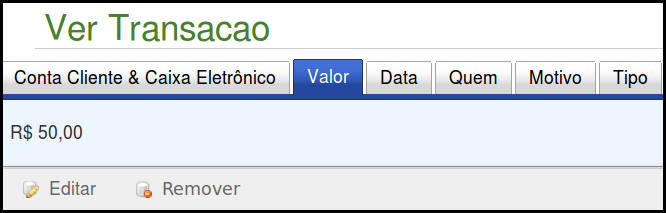
\includegraphics[width=12cm]{abas}
\caption{Visão {\bf transacao/show.gsp}: visualização em abas}
\label{abasFig}
\end{figure}

\vspace{0.4cm}

\item A {\it tag} {\bf  <richui:tabContent>} (linhas 39-81) define o conteúdo de
  cada  aba. Ao  selecionar  uma aba,  o  conteúdo da  aba  é apresentado.   Por
  exemplo, O conteúdo da aba {\bf Valor} é apresentado na Figura~\ref{abasFig}.  

\vspace{0.4cm}

\item No caso  da aba {\bf Conta Cliente \& Caixa  Eletrônico}, foi utilizado um
  menu {\it accordion}.  O menu {\it accordion} é definido pelas {\it tags} {\bf
    <richui:accordion>}      e     {\bf      <richui:accordionItem>}     (linhas
  41-54). Figura~\ref{accordionFig} apresenta as  duas opções disponíveis da aba
  {\bf Conta Cliente \& Caixa Eletrônico}. 

\end{itemize}

\vspace{0.5cm}

\begin{figure}[htbp]
\centering
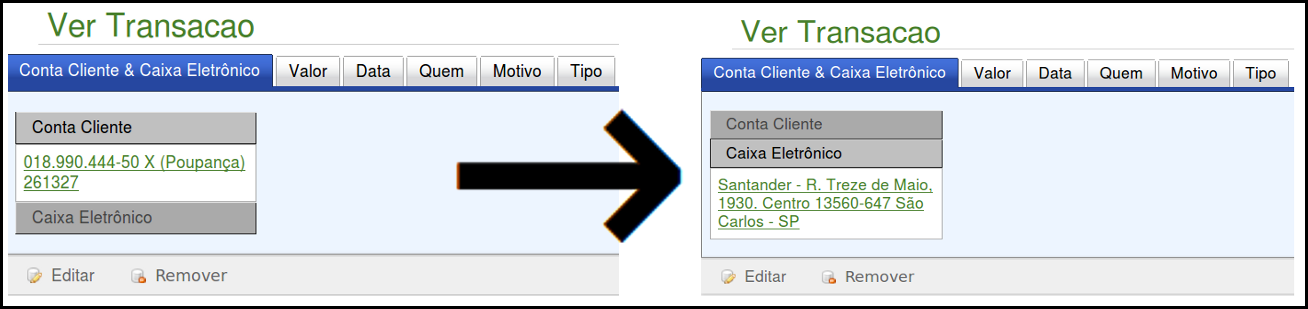
\includegraphics[width=14cm]{accordion}
\caption{Visão {\bf transacao/show.gsp}: menu {\it accordion}}
\label{accordionFig}
\end{figure}

\vspace{0.5cm}

\begin{lstlisting}[caption={\it     Template}     {\bf    transacao/\_form.gsp},
    frame=trBL, float=htbp, label=codTransacaoShow2, numbers=left]
<%@ page import="br.ufscar.dc.dsw.Transacao" %>
<!DOCTYPE html>
<html>
 <head>
  <meta name="layout" content="main">
   <g:set var="entityName" value="${message(code: 'transacao.label', default: 'Transacao')}" />
   <title><g:message code="default.show.label" args="[entityName]" /></title>
   <r:require module="pure-all" />
   <resource:tabView />
   <resource:accordion skin="default" />
 </head>
 <body>
  <a href="#show-transacao" class="skip" tabindex="-1">
  <g:message code="default.link.skip.label" default="Skip to content&hellip;"/></a>
  <div class="pure-menu pure-menu-open pure-menu-horizontal">
   <ul>
    <li><a class="home" href="${createLink(uri: '/')}"><g:message code="default.home.label"/></a></li>
    <li><g:link class="list" action="index"><g:message code="default.list.label" args="[entityName]"/></g:link>
    </li><li><sec:access controller="transacao" action='create'>
         <g:link class="create" action="create"><g:message code="default.new.label" args="[entityName]" /></g:link>
        </sec:access></li>
    <li><g:link controller="logout">Logout</g:link></li>
   </ul>
  </div>
  <div id="show-transacao" class="content scaffold-show" role="main">
   <h1><g:message code="default.show.label" args="[entityName]" /></h1>
   <g:if test="${flash.message}">
    <div class="message" role="status">${flash.message}</div>
   </g:if>
   <richui:tabView id="tabView">
    <richui:tabLabels>
     <richui:tabLabel selected="true" title="${message(code:'transacao.main')}" />
     <richui:tabLabel title="${message(code:'transacao.value')}" />
     <richui:tabLabel title="${message(code:'transacao.data')}" />
     <richui:tabLabel title="${message(code:'transacao.quem')}" />
     <richui:tabLabel title="${message(code:'transacao.motivo')}" />
     <richui:tabLabel title="${message(code:'transacao.tipo')}" />
    </richui:tabLabels>
    <richui:tabContents>
     <richui:tabContent>
      <richui:accordion>
       <richui:accordionItem id="1" caption="Conta Cliente">
        <g:if test="${transacaoInstance?.contaCliente}">
         <g:link controller="contaCliente" action="show" id="${transacaoInstance?.contaCliente?.id}">
                            ${transacaoInstance?.contaCliente?.encodeAsHTML()}</g:link>
        </g:if>
       </richui:accordionItem>
       <richui:accordionItem caption="Caixa Eletr^ô^nico">
        <g:if test="${transacaoInstance?.caixaEletronico}">
         <g:link controller="caixaEletronico" action="show" id="${transacaoInstance?.caixaEletronico?.id}">
                            ${transacaoInstance?.caixaEletronico?.encodeAsHTML()}</g:link>
        </g:if>
       </richui:accordionItem>
      </richui:accordion>
     </richui:tabContent>
     <richui:tabContent>
      <g:if test="${transacaoInstance?.valor}">                        
       <g:formatNumber number="${transacaoInstance.valor}" type="currency" />
      </g:if>
     </richui:tabContent>
     <richui:tabContent>
      <g:if test="${transacaoInstance?.data}">
       <g:formatDate date="${transacaoInstance?.data}" type="datetime" style="LONG" timeStyle="SHORT"/>
      </g:if>
     </richui:tabContent>
     <richui:tabContent>
      <g:if test="${transacaoInstance?.quem}">
       <g:fieldValue bean="${transacaoInstance}" field="quem"/>
      </g:if>
     </richui:tabContent>
     <richui:tabContent>
      <g:if test="${transacaoInstance?.motivo}">
       <g:fieldValue bean="${transacaoInstance}" field="motivo"/>
      </g:if>
     </richui:tabContent>
     <richui:tabContent>
      <g:if test="${transacaoInstance?.tipo}">
       <g:fieldValue bean="${transacaoInstance}" field="tipo"/></span>
      </g:if>
     </richui:tabContent>
    </richui:tabContents>
   </richui:tabView>    
   <g:form url="[resource:transacaoInstance, action:'delete']" method="DELETE">
    <fieldset class="buttons">
     <sec:access controller="transacao" action='edit'>
      <g:link class="edit" action="edit" resource="${transacaoInstance}">
              <g:message code="default.button.edit.label" default="Edit" /></g:link>
     </sec:access>
     <sec:access controller="transacao" action='delete'>
      <g:actionSubmit class="delete" action="delete" value="${message(code: 'default.button.delete.label', 
         default: 'Delete')}" onclick="return confirm('${message(code: 'default.button.delete.confirm.message', 
         default: 'Are you sure?')}');" />
     </sec:access>
    </fieldset>
   </g:form>
  </div>
 </body>
</html>
\end{lstlisting}

\newpage

\section{Extratos Bancários}

\vspace{0.5cm}

O  controlador  {\bf ExtratoController}  é  responsávela  pela implementação  da
funcionalidade de  visualização e impressão de extratos  bancários associados às
contas bancárias.  A implementação desse controlador  encontra-se apresentada no
Código~\ref{codExtratoController}. 

\begin{lstlisting}[caption=  Controlador  {\bf  ExtratoController},  frame=trBL,
    float=htbp, label=codExtratoController, numbers=left] 
package br.ufscar.dc.dsw
import java.text.SimpleDateFormat
import org.springframework.security.access.annotation.Secured

@Secured('ROLE_CLIENTE')
class ExtratoController { 

    def index() {
        def linhas = getLinhas()
        if(params?.format && params.format == "pdf"){
            render( filename:"extrato.pdf",
                view:"/extrato/_pdf",
                model:[lines: linhas, contaCliente:session.contaCliente],
                marginLeft:20,
                marginTop:35,
                marginBottom:20,
                marginRight:20,
                headerSpacing:10,
            )   
        }
        model:[lines: linhas]
    }
    
    def chart = {
        def columns = [['date', 'Dia'], ['number', 'Saldo (R$)']]
        def lines = []
        def linhas = getLinhas()
        def anterior = null
        SimpleDateFormat formato = new SimpleDateFormat("dd/MM/yyyy")

        linhas.reverse().each {
            def atual = formato.format(it.data)
            if (!atual.equals(anterior)) {
                lines.add([it.data, it.saldo])                
            }
            anterior = it.data
        }
          
        ["columns": columns, "lines": lines]
    }

    private List<Line> getLinhas() {
        def conta = Conta.get(session.contaCliente.conta.id)
        def saldo = conta.saldo
        def results = Transacao.findAllByContaCliente(session.contaCliente, [sort:"data"])
        results.each {
            saldo -= it.getValorReal()
        }

        List<Line> linhas = new ArrayList<Line>();
        Line linha = new Line(session.contaCliente.conta.abertura, "ABERTURA", saldo)
        linhas.add(linha)       

        results.each {
            saldo += it.getValorReal()
            linha = new Line(it.data, it.tipo, saldo, it.valor, it.motivo)
            linhas.add(linha)
        }

        linha = new Line(new Date(), "SALDO ATUAL", saldo)
        linhas.add(linha)
        return linhas
    }
}
\end{lstlisting} 

\vspace{0.5cm}

\begin{itemize}

\item A  ação {\bf index()}  (linhas 7-21) simplesmente invoca  implicitamente a
  visão {\bf  index.gsp} (Código~\ref{codExtratoIndex}) que  representa extratos
  bancários em formato HTML.   Adicionalmente, essa ação renderiza, utilizando o
  {\it plugin}  {\bf wkhtmltopdf}, o  arquivo {\bf extrato.pdf} baseado  no {\it
    template}  {\bf extrato/\_pdf.gsp} (Código~\ref{codPdfTemplate}).   Ou seja,
  essa ação é também responsável  por gerar os arquivos que representam extratos
  bancários em formato PDF; 

\vspace{0.5cm}

\item A ação  {\bf chart()} (linhas 23-38) simplesmente  invoca implicitamente a
  visão   {\bf  chart.gsp}   (Código~\ref{codChart})  que   será   discutida  na
  Seção~\ref{secExtratoVisoes};

\vspace{0.5cm} 

\item  É importante salientar  que as  ações (e  respectivas visões)  utilizam o
  método  privado  {\bf  getLinhas()}   (linhas  40-58)  retorna  uma  lista  de
  instâncias  da classe  {\bf  Line}.   Conforme pode-se  observar,  a lista  de
  instâncias da classe  {\bf Line} é construída através da  iteração da lista de
  transações (ordenadas pela data) associadas às contas bancárias; 

\vspace{0.5cm}

\item      A     classe      Java     {\bf      Line}\footnote{Arquivo:     {\bf
    src/br/ufscar/dc/dsw/Line.java}}    (Código~\ref{codLine})    armazena    as
  informações (atributos:  {\bf data}, {\bf  tipo}, {\bf motivo}, {\bf  valor} e
  {\bf saldo})  relacionadas às  transações e representa  cada linha  do extrato
  bancário a ser visualizado e/ou impresso.  

\end{itemize}

\vspace{0.5cm}

\begin{lstlisting}[caption=Classe  Java   {\bf  Line},  frame=trBL,  float=htbp,
    label=codLine] 
package br.ufscar.dc.dsw;

import java.util.Date;

public class Line implements Comparable<Line>{
    
    private final Date data;
    
    private final String tipo;
    
    private final String motivo;
    
    private final Double valor;
    
    private final Double saldo;

    public Line(Date data, String tipo, Double saldo, Double valor, String motivo) {
        this.data = data;
        this.tipo = tipo;
        this.saldo = saldo;
        this.valor = valor;
        this.motivo = motivo;
    }
    
    public Line(Date data, String tipo, double saldo) {
        this(data, tipo, saldo, null, null);
    }
    

    public Date getData() {
        return data;
    }

    public String getTipo() {
        return tipo;
    }

    public String getMotivo() {
        return motivo;
    }

    public Double getValor() {
        return valor;
    }

    public Double getSaldo() {
        return saldo;
    }    

    
    @Override
    public int compareTo(Line o) {
        return this.data.compareTo(o.data);
    }

    @Override
    public String toString() {
        return data.toString() + " - " + valor + " - " + saldo;
    }
    
}
\end{lstlisting}

\newpage

\subsection{Visões}\label{secExtratoVisoes}

\vspace{0.5cm}

Relembrando   a   discussão  da   Seção~\ref{secEstatico},   para  cada   método
correspondente a  uma ação em um  controlador é criada  uma correspondente visão
(arquivo  com  extensão {\bf  .gsp}).   Assim, a  ação  {\bf  index()}, de  {\bf
  ExtratoController},  tem  o  correspondente  {\bf  index.gsp}  que  representa
extratos  bancários em  formato HTML.  A implementação  dessa  visão encontra-se
apresentada no Código~\ref{codExtratoIndex}.

\vspace{0.3cm}

\noindent  Figura~\ref{figExtratoHTML}  apresenta   um  exemplo  de  um  extrato
bancário representado pela visão {\bf extrato/index.gsp}. É importante salientar
que essa visão  já apresenta um leiaute mais  responsivo: menu horizontal (linha
14) e tabela (linha 26). 

\vspace{0.2cm}

\begin{lstlisting}[caption=Visão {\bf extrato/index.gsp}, frame=trBL, float=htbp,
    label=codExtratoIndex, numbers=left]
<%@ page import="org.grails.plugins.google.visualization.data.Cell; 
                 org.grails.plugins.google.visualization.util.DateUtil" %>
<%@ page import="br.ufscar.dc.dsw.Transacao" %>
<!DOCTYPE html>
<html>
  <head>
    <meta name="layout" content="main">
    <title><g:message code="extrato.statement"/></title>
    <r:require module="pure-all" />
  </head>
  <body>
    <a href="#list-transacao" class="skip" tabindex="-1">
    <g:message code="default.link.skip.label" default="Skip to content&hellip;"/></a>
    <div class="pure-menu pure-menu-open pure-menu-horizontal">
      <ul>
        <li><a class="home" href="${createLink(uri: '/')}"><g:message code="default.home.label"/></a></li>
        <li><g:link action="chart"><g:message code="extrato.chart" default="Chart" /></g:link></li>
        <li><g:link controller="logout">Logout</g:link></li>
      </ul>
    </div>
    <div id="list-transacao" class="content scaffold-list" role="main">
      <h1><g:message code="extrato.statement"/></h1>
      <g:if test="${flash.message}">
        <div class="message" role="status">${flash.message}</div>
      </g:if>
      <table class="pure-table pure-table-bordered">
        <thead>
          <tr>
            <th><g:message code="transacao.data"/></th>
            <th><g:message code="transacao.tipo"/></th>
            <th><g:message code="transacao.motivo"/></th>
            <th><g:message code="extrato.valor"/></th>
            <th><g:message code="extrato.saldo"/></th>
          </tr>
        </thead>
        <tbody>
          <g:each in="${lines}" status="i" var="linha">
            <tr class="${(i % 2) == 0 ? 'even' : 'odd'}">
             <td><g:formatDate date="${linha.data}" type="date" style="SHORT"/></td>
             <td>${fieldValue(bean: linha, field: "tipo")}</td>
             <td>${fieldValue(bean: linha, field: "motivo")}</td>
             <td><g:formatNumber number="${linha.valor}" type="currency" /></td>
             <td><g:formatNumber number="${linha.saldo}" type="currency" /></td>
            </tr>
          </g:each>
        </tbody>
      </table>
      <center>
        <h4>
          <g:message code="extrato.saveaspdf"/>
          <g:link action="index.pdf">
            <img src="${resource(dir: 'images', file: 'pdf.jpg')}" alt="PDF" width="18px"/>
          </g:link>
        </h4>
      </center>
    </div>
  </body>
</html>
\end{lstlisting}

\vspace{0.2cm}

\noindent Em  complemento, essa visão adiciona  um {\it link}  (linha 51-53) que
possibilita salvar o extrato em  formato PDF. Conforme pode-se observar que esse
{\it  link} invoca  a ação  {\bf index}  do controlador  {\bf ExtratoController}
passando o parâmetro {\bf format} com o  valor igual a {\bf pdf}.  Nesse caso, o
controlador {\bf  ExtratoController} renderiza,  utilizando o {\it  plugin} {\bf
  wkhtmltopdf},  o arquivo  {\bf  extrato.pdf} baseado  no  {\it template}  {\bf
  extrato/\_pdf.gsp}.

\begin{figure}[htbp]
\centering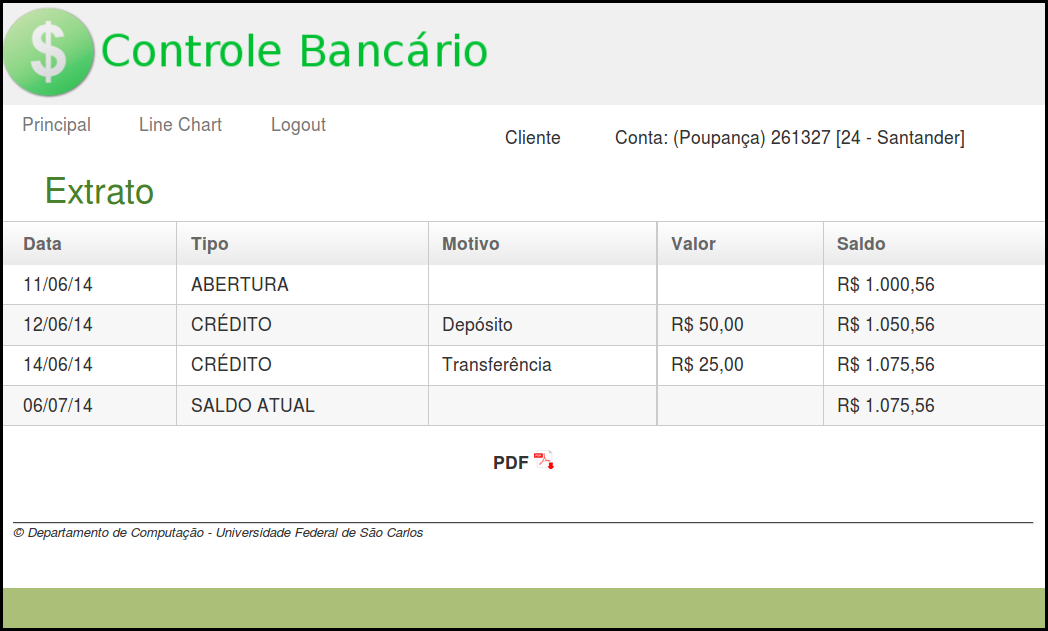
\includegraphics[width=12cm]{extrato}
\caption{Extrato Bancário em formato HTML}
\label{figExtratoHTML}
\end{figure}

Conforme   pode-se   observar,   o   {\it  template}   {\bf   extrato/\_pdf.gsp}
(Código~\ref{codPdfTemplate}) define  uma página HTML que será  convertida em um
arquivo  PDF.  Figura~\ref{figExtratoPDF}  apresenta  um exemplo  de um  extrato
bancário, em formato PDF, gerado pela ação {\bf index()}.

\begin{figure}[h]
\centering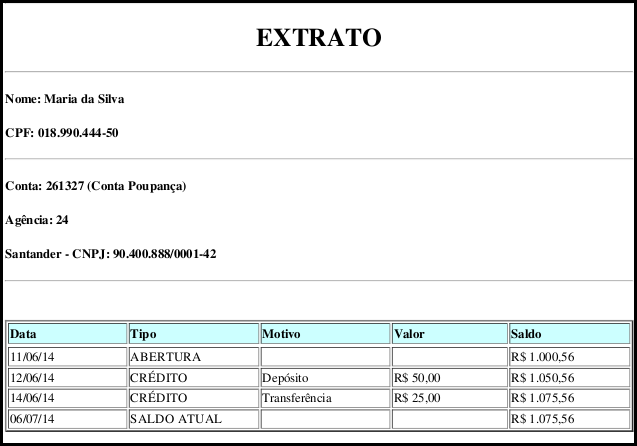
\includegraphics[width=11cm]{extratoPDF}
\caption{Extrato Bancário em formato PDF}
\label{figExtratoPDF}
\end{figure}

\newpage

\begin{lstlisting}[caption={\it Template} {\bf extrato/\_pdf.gsp}, frame=trBL,
    label=codPdfTemplate]
<%@ page import="br.ufscar.dc.dsw.ContaCorrente" %>
<%@ page import="br.ufscar.dc.dsw.ClienteFisico" %>
<hr/>
<center>
  <h1>EXTRATO</h1>
</center>
<hr/>
<h4>Nome: ${contaCliente.cliente.nome}</h4>
<h4>
  ${contaCliente.cliente instanceof ClienteFisico ? "CPF: " + contaCliente.cliente.CPF : 
                                                    "CNPJ: " + contaCliente.cliente.CNPJ}
</h4>
<hr/>
<h4>Conta: ${contaCliente.conta.numero}
  (${contaCliente.conta instanceof ContaCorrente ? "Conta Corrente" : "Conta Poupan^ç^a"})</h4>
<h4>Ag^ê^ncia: ${contaCliente.conta.agencia.numero}</h4>
<h4>${contaCliente.conta.agencia.banco} - CNPJ: ${contaCliente.conta.agencia.banco.CNPJ}</h4>
<hr/>
<br/>
<br/>
<table style="text-align: left; margin-left: auto; margin-right: auto;" class="pure-table pure-table-bordered" 
       border="2">
  <thead> 
    <tr>
      <th style="width: 200px; background-color: rgb(204, 255, 255);">Data</th>
      <th style="width: 200px; background-color: rgb(204, 255, 255);">Tipo</th>
      <th style="width: 200px; background-color: rgb(204, 255, 255);">Motivo</th>
      <th style="width: 200px; background-color: rgb(204, 255, 255);">Valor</th>
      <th style="width: 200px; background-color: rgb(204, 255, 255);">Saldo</th>
    </tr>
   </thead> 
   <tbody>
     <g:each in="${lines}" status="i" var="linha"> 
       <tr class="${(i % 2) == 0 ? 'even' : 'odd'}">
         <td><g:formatDate date="${linha.data}" type="date"/></td>
         <td>${fieldValue(bean: linha, field: "tipo")}</td>
         <td>${fieldValue(bean: linha, field: "motivo")}</td>
         <td><g:formatNumber number="${linha.valor}" type="currency"/></td>
         <td><g:formatNumber number="${linha.saldo}" type="currency"/></td>
       </tr>
     </g:each>
   </tbody>
</table>
<br/>
<br/>
<hr/>
<center>
  <h6>&copy; Departamento de Computa^çã^o - Universidade Federal de S^ã^o Carlos</h6>
  <h6><g:formatDate date="${new Date()}" type="datetime" style="LONG"/></h6>
</center>
\end{lstlisting}

A  visão  {\bf extrato/chart.gsp}  renderiza,  utilizando  o  {\it plugin}  {\bf
  google-visualization},  um gráfico  de  linhas que  representa a  movimentação
financeira  das  contas  bancárias.  A  implementação  dessa  visão  encontra-se
apresentada no Código~\ref{codChart}.  

\vspace{0.3cm}

\noindent  Conforme  pode-se  observar  essa  visão utiliza  a  {\it  tag}  {\bf
  <gvisualization:lineCoreChart>} para gerar um gráfico de linhas com os valores
({\bf columns} e {\bf lines}) retornados pela ação {\bf chart()}.  

\vspace{0.4cm}

\begin{lstlisting}[caption=Visão {\bf extrato/chart.gsp}, frame=trBL,
    label=codChart]
<%@ page import="org.grails.plugins.google.visualization.data.Cell; 
                 org.grails.plugins.google.visualization.util.DateUtil" %>
<html>
  <head>
    <title>Movimenta^çã^o Financeira</title>
    <meta name="layout" content="main" />
    <gvisualization:apiImport/>
    <r:require module="pure-all" />
  </head>
  <body>
    <div class="pure-menu pure-menu-open pure-menu-horizontal">
      <ul>
        <li><a class="home" href="${createLink(uri: '/')}"><g:message code="default.home.label"/></a></li>
        <li><g:link controller="extrato"><g:message code="extrato.statement"/></g:link></li>
        <li><g:link controller="logout">Logout</g:link></li>
      </ul>
    </div>
    <div id="list-transacao" class="content scaffold-list" role="main">
       <div id="linechart"></div>
       <gvisualization:lineCoreChart elementId="linechart" width="${800}" height="${300}" 
                      title="Movimenta^çã^o Financeira" columns="${columns}" data="${lines}" />
    </div>
  </body>
</html>
\end{lstlisting}

\newpage

\noindent   Figura~\ref{figLineChart}  apresenta  um   exemplo  de   um  gráfico
renderizado  pela ação  {\bf chart.gsp}.   Esse gráfico  ilustra  a movimentação
financeira (créditos e débitos) de uma conta bancária.

\vspace{0.3cm}

\begin{figure}[h]
\centering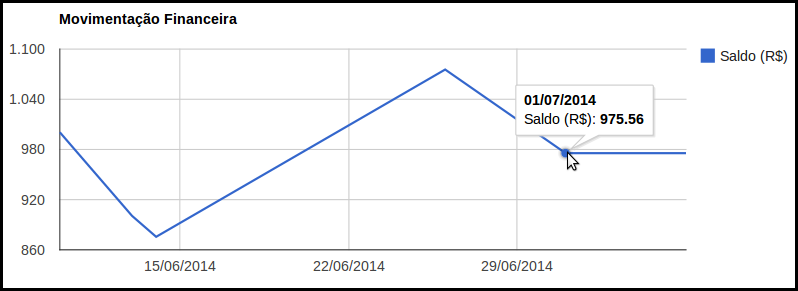
\includegraphics[width=14cm]{lineChart}
\caption{Movimentação financeira das contas bancárias}
\label{figLineChart}
\end{figure}

\section{Internacionalização - Mensagens I18n}
\index{Internacionalização~-~I18n}

\vspace{0.5cm}

Conforme pode-se observar pelas visões apresentadas/discutidas nesse capítulo, a
{\it tag} {\bf <g:message>} é utilizada para inserir rótulos internacionalizados
nessas  visões.  Dessa  forma, é  necessário adicionar  uma tradução,  para cada
idioma desejado, desses rótulos nos arquivos presentes no diretório {\bf i18n}. 

\vspace{0.2cm}

\noindent  Figura~\ref{figI18n} apresenta  a tradução  desses rótulos  que foram
inseridos  no arquivo  {\bf messages\_pt\_BR.properties}  ({\it  Message Bundle}
para o Português do Brasil).  

\vspace{0.3cm}

\begin{figure}[htbp]
\begin{mdframed}
\begin{footnotesize}
\begin{verbatim}
# Visão cliente/index.gsp
search.label=Busca de Cliente

# Visão main/index.gsp
main.options = Opções

# Visões - Controlador Transacao
transacao.main  = Conta Cliente & Caixa Eletrônico
transacao.value = Valor
transacao.data = Data
transacao.quem = Quem
transacao.motivo = Motivo
transacao.tipo = Tipo

# Visões - Controlador Extrato
extrato.statement = Extrato
extrato.chart = Line Chart
extrato.valor = Valor
extrato.saldo = Saldo
extrato.saveaspdf = PDF
\end{verbatim}
\end{footnotesize}
\end{mdframed}
\caption{Mensagens internacionalizadas}
\label{figI18n}
\end{figure}

\newpage

\section{Serviço {\it web} REST}\label{secWebREST}
\index{Serviços {\it web} REST}

\vspace{0.5cm}

REST  não é  uma tecnologia  em si,  pode ser  considerada mais  como  um padrão
arquitetural. O padrão arquitetural REST é  muito simples e envolve apenas o uso
simples de  XML ou  JSON como meio  de comunicação,  em conjunto com  padrões na
definição de  URLs que são  ``representações'' do sistema subjacente,  e métodos
HTTP, como GET, PUT,  POST e DELETE. Cada método HTTP é  mapeado para um tipo de
ação  do controlador.  Por exemplo,  o método  GET é  mapeado para  operações de
recuperação, o método  PUT é mapeado para operações de criação,  o método POST é
mapeado para operações de atualização e  assim por diante. Neste sentido REST se
encaixa muito bem com as operações CRUD. 

\vspace{0.2cm}

\noindent Essa seção  descreve a implementação de um serviço  {\it web} REST que
retorna uma lista  (em formato JSON ou XML) de agências  de um determinado banco
(parâmetro {\bf numero}). O controlador {\bf AgenciaController} é a escolha mais
óbvia para ser o responsável  por prover essa nova funcionalidade.  Dessa forma,
Código~\ref{codAgenciaController2}  apresenta  a   implementação  da  ação  {\bf
  list()},   do   controlador    {\bf   AgenciaController},   responsável   pela
implementação do serviço {\it web}  REST. Por questão de brevidade, apenas serão
apresentadas as mudanças realizadas nesse controlador.

\vspace{0.5cm}

\begin{lstlisting}[caption=Controlador  {\bf AgenciaController},  frame  = trBL,
    float=htbp, label=codAgenciaController2] 
import grails.converters.JSON
import grails.converters.XML

// Demais imports do controlador AgenciaController

class AgenciaController { 

    // Demais a^çõ^es/atributos/m^é^todos do controlador AgenciaController
   
    @Secured('IS_AUTHENTICATED_ANONYMOUSLY')
    def list() {
        
        def banco = Banco.findAllByNumero(params.numero)
        def agencias = Agencia.findAllByBanco(banco)
        def estado = Estado.findBySigla(params.estado)
        def cidade = Cidade.findByNomeAndEstado(params.cidade, estado)
        
        List<Info> lista = new ArrayList<Info>()
        
        agencias.each {
            
            if (!params.cidade || it.endereco.cidade == cidade) {
                Info info = new Info(it.banco.nome, it.numero, 
                    it.nome, it.endereco.toString())
            
                lista.add(info)
            }
        }
            
        withFormat {
            json { render lista as JSON }
            xml { render lista as XML }
        }
    }
}
\end{lstlisting}

\begin{itemize}

\vspace{0.5cm}

\item  A anotação  {\bf  @Secured('IS\_AUTHENTICATED\_ANONYMOUSLY')} indica  que
  esse serviço {\it web} é público e pode ser acessado por qualquer usuário e/ou
  aplicação.  

\vspace{0.5cm} 

\item  É importante  salientar que  a  ação {\bf  list()} retorna  uma lista  de
  instâncias  da classe  {\bf  Info}.   Conforme pode-se  observar,  a lista  de
  instâncias da classe  {\bf Info} é construída através da  iteração da lista de
  agências    associadas    a    um    determinado   banco    (parâmetro    {\bf
    numero}).   Opcionalmente,  a ação  {\bf  list()}  pode  filtrar essa  lista
  visando  apenas  retornar  as  agências  situadas em  uma  determinada  cidade
  (parâmetros {\bf cidade} e {\bf estado}); 

\vspace{0.5cm}

\item      A     classe      Java     {\bf      Info}\footnote{Arquivo:     {\bf
    src/br/ufscar/dc/dsw/Info.java}}    (Código~\ref{codInfo})    armazena    as
  informações  (atributos:  {\bf numero},  {\bf  nome},  {\bf  endereco} e  {\bf
    banco}) relacionadas às agências bancárias.  

\vspace{0.5cm}

\item Por  fim, a ação {\bf  list()} constrói a  saída ao renderizar a  lista de
  instâncias da classe {\bf Info} (em formato JSON ou XML).  A conversão para os
  formatos JSON ou XML é realizada  através da utilização das classes {\bf JSON}
  e {\bf XML} do pacote {\bf grails.converters}. 

\end{itemize}

\begin{lstlisting}[caption=Classe  Java   {\bf  Info},  frame=trBL,  float=htbp,
    label=codInfo] 
package br.ufscar.dc.dsw;

public class Info {
    
    private final int numero;

    private final String nome;

    private final String endereco;

    private final String banco;

    public Info(String banco, int numero, String nome, String endereco) {
        this.banco = banco;
        this.numero = numero;
        this.nome = nome;
        this.endereco = endereco;
    }

    public String getBanco() {
        return banco;
    }

    public String getEndereco() {
        return endereco;
    }

    public String getNome() {
        return nome;
    }

    public int getNumero() {
        return numero;
    }
    
    
}
\end{lstlisting}

Figura~\ref{figJSON} ilustra  o acesso  desse serviço {\it  web} através  da URL
{\footnotesize\url{http://localhost:8080/ControleBancarioV4/agencia/list.json?numero=1}}.
É importante salientar  que essa URL define a ação a  ser acessada: {\bf list()}
do controlador {\bf AgenciaController}.  Adicionalmente, essa URL define o valor
do parâmetro {\bf numero} e o formato da resposta (formato JSON).

\vspace{0.5cm}

\begin{figure}[h]
\centering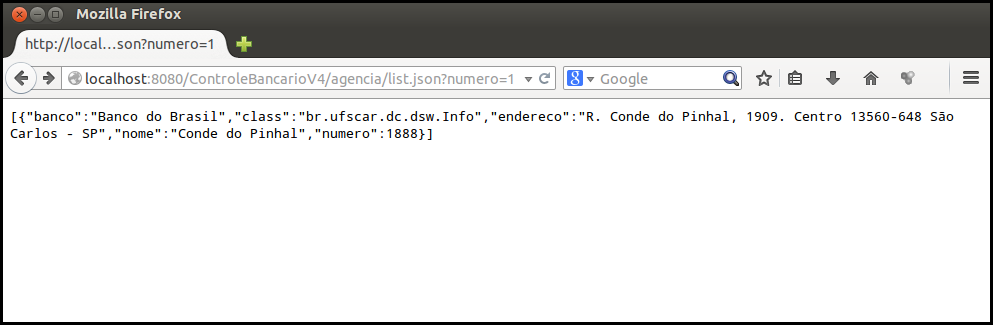
\includegraphics[width=15cm]{restJSON}
\caption{Serviço {\it web} REST: Formato JSON}
\label{figJSON}
\end{figure}

Analogamente, Figura~\ref{figXML} ilustra o acesso desse serviço {\it web} através da URL
{\footnotesize\url{http://localhost:8080/ControleBancarioV4/agencia/list.xml?numero=1}}. 
Novamente  essa URL define  a ação  a ser  acessada, o  valor do  parâmetro {\bf
  numero} e o formato da resposta (formato XML). 

\vspace{0.5cm}

\begin{figure}[h]
\centering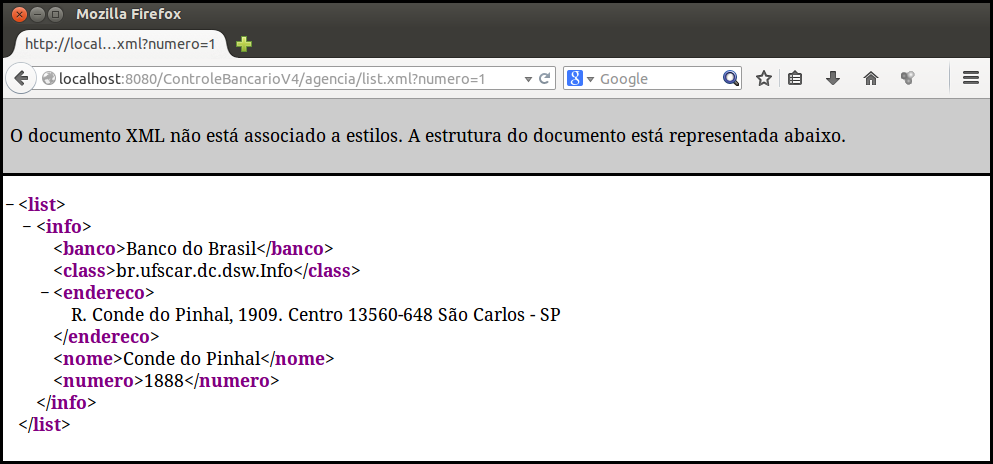
\includegraphics[width=15cm]{restXML}
\caption{Serviço {\it web} REST: Formato XML}
\label{figXML}
\end{figure}

\section{Considerações finais}

\vspace{0.3cm}


Esse  capítulo apresentou  a quarta  versão da  implementação da  aplicação {\bf
  ControleBancario}.         O        código-fonte        dessa        aplicação
({\footnotesize\texttt{ControleBancarioV4.zip}}) encontra-se  disponível no {\it
  Moodle}         do        curso,        localizado         no        endereço:
{\footnotesize\url{http://moodle.latosensu.dc.ufscar.br}}. Seguindo os passos do
tutorial   apresentado   obtem-se   esse   mesmo  código   da   aplicação   {\bf
  ControleBancario}.  


